\chapter{HSV}

HSV (Hue, Saturation, Value) is a different representation of the RGB (Red, Green, Blue) color-model. It is used to make easy adjustments according to it's components. Usually image programs and \LaTeX \space interpret images as RGB images. This is the reason for the colorful representation of the images.

\section{Performance Tests}

The RGB2HSV is also performing best (between $ 6.27 $ and $ 43.51 $) with a parallelization on the outer For-Loop.  Strongly improving until the usage of 4 threads. Using 8 threads yields the performance peak. Same observations as in the grayscale performance tests \ref{fig:grayscale} were made, when to many threads were in use.

\begin{center}
    \begin{figure}[H]
        \centering

        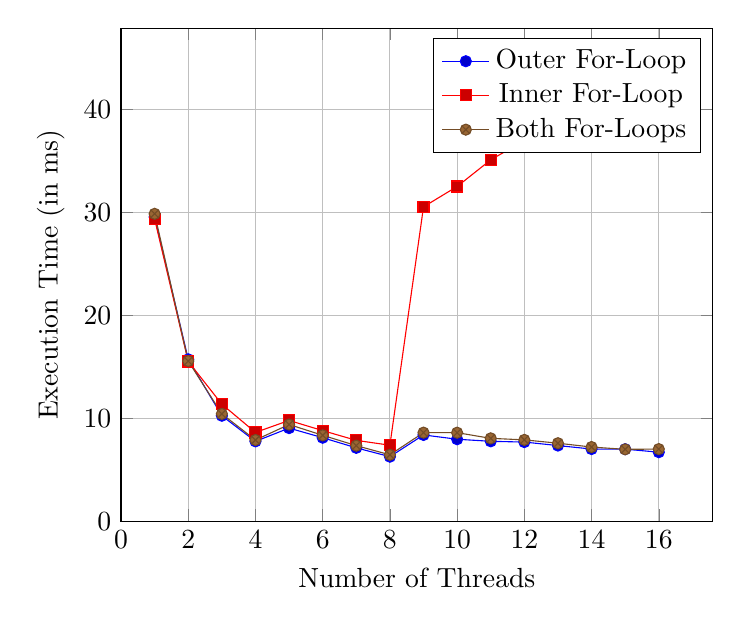
\begin{tikzpicture}
            \begin{axis}[
                title={},
                width=0.75\textwidth,
                xlabel={Number of Threads},
                ylabel={Execution Time (in ms)},
                xmin=0,
                ymin=0,
                grid=major
            ]
                \addplot coordinates {
                    (1,29.5366)(2,15.7231)(3,10.2453)(4,7.7598)(5,9.04545)(6,8.11285)(7,7.1297)(8,6.27195)(9,8.3824)(10,7.96645)(11,7.7646)(12,7.69085)(13,7.35195)(14,7.01335)(15,7.00095)(16,6.70895)
                };
                \addlegendentry{Outer For-Loop}

                \addplot coordinates {
                    (1,29.3423)(2,15.5132)(3,11.3651)(4,8.62715)(5,9.78995)(6,8.8026)(7,7.857)(8,7.38445)(9,30.5217)(10,32.4977)(11,35.0829)(12,36.9657)(13,37.1315)(14,39.4836)(15,39.4552)(16,43.51)
                };
                \addlegendentry{Inner For-Loop}
                
                \addplot coordinates {
                    (1,29.8459)(2,15.5525)(3,10.4249)(4,7.89)(5,9.39475)(6,8.3478)(7,7.3445)(8,6.45355)(9,8.6068)(10,8.60125)(11,8.05395)(12,7.9041)(13,7.581)(14,7.2079)(15,6.9847)(16,7.01045)
                };
                \addlegendentry{Both For-Loops}   
            \end{axis}
        \end{tikzpicture}
        \caption{RGB to HSV Performance Tests}
    \end{figure}
\end{center}

\section{Results}

The self-implemented algorithm yields very similar results compared to the OpenCV version. Subtracting the image matrices reveals a small differences, which could be the consequences of rounding-errors.

\begin{figure}[H]
    \centering

    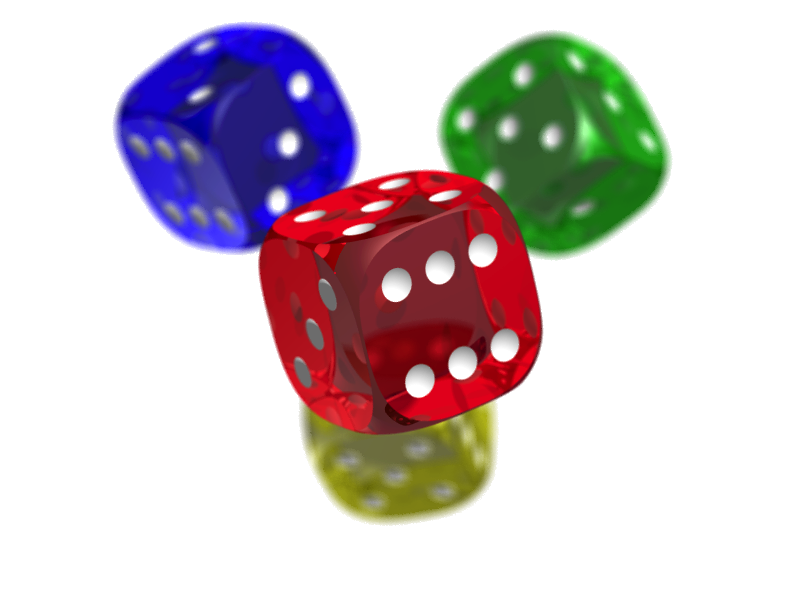
\includegraphics[width=0.20\textwidth]{images/dice.png}
    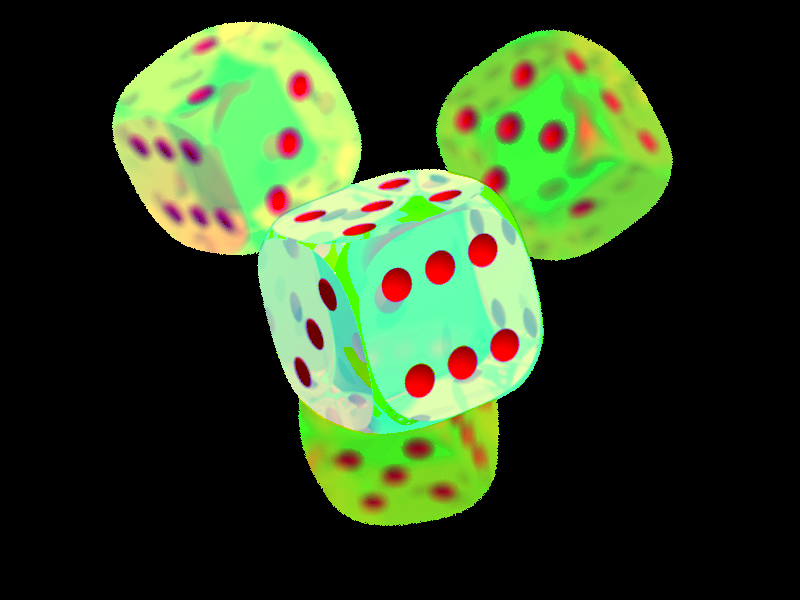
\includegraphics[width=0.20\textwidth]{images/cv-hsv.png}
    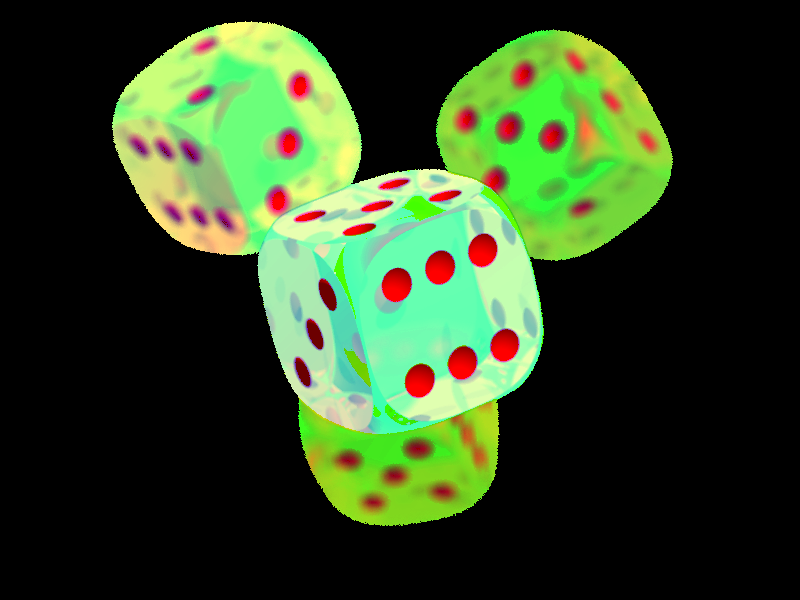
\includegraphics[width=0.20\textwidth]{images/own-hsv.png}
    
    \caption{RGB to HSV results of OpenCV (middle) and self-implemented  Algorithm (right)}
    \label{fig:hsv}
\end{figure}

\section{Implementation}

\begin{listing}[H]
    \begin{minted}{cpp}
cv::Mat applyHsvOuter(cv::Mat srcImage, int numThreads = omp_get_num_procs()) {
    cv::Mat destImage(srcImage.rows, srcImage.cols, CV_8UC3);
    omp_set_num_threads(numThreads);

    #pragma omp parallel for default(none) shared(srcImage, destImage)
    for (int row = 0; row < srcImage.rows; row++) {
        for (int col = 0; col < srcImage.cols; col++) {
            auto srcPixel = srcImage.at<cv::Vec3b>(row, col);

            double r = srcPixel[2] / 255.0;
            double g = srcPixel[1] / 255.0;
            double b = srcPixel[0] / 255.0;

            double h, s, v;

            double cMax = std::max(std::max(r, g), b);
            double cMin = std::min(std::min(r, g), b);
            double diff = cMax - cMin;

            if (cMax == cMin) {
                h = 0;
            } else if (cMax == r) {
                h = int(60 * ((g - b) / diff) + 360) % 360;
            } else if (cMax == g) {
                h = int(60 * ((b - r) / diff) + 120) % 360;
            } else {
                h = int(60 * ((r - g) / diff) + 240) % 360;
            }

            s = cMax == 0 ? 0 : (diff / cMax);
            v = cMax;

            cv::Vec3b destPixel = cv::Vec3b(
                    uchar(h / 360.0 * 180.0),
                    uchar(s * 255.0),
                    uchar(v * 255.0)
            );

            destImage.at<cv::Vec3b>(row, col) = destPixel;
        }
    }

    return destImage;
}
    \end{minted}
    \captionof{lstlisting}{RGB to HSV conversion with parallelization of the outer For-Loop}
    \label{listing:hsv}
\end{listing}

\section{Comparison with OpenCV}

\subsection{Code}

\noindent
As with grayscale image transformation to HSV can be done in one line of code with OpenCV. 

\begin{listing}[H]
    \begin{minted}{cpp}
cv::cvtColor(srcImage, destImage, cv::COLOR_BGR2HSV);
    \end{minted}
    \captionof{lstlisting}{RGB to HSV conversion  with OpenCV}
    \label{listing:hsv_opencv}
\end{listing}

\subsection{Performance}

OpenCV outperforms the self-implemented version significantly with a runtime of $ 0.16 $ ms .